\documentclass[12pt]{article}

\usepackage{baseset}
\DeclareSymbolFont{operators}{OT1}{ntxtlf}{m}{n}
\SetSymbolFont{operators}{bold}{OT1}{ntxtlf}{b}{n}
\newcommand{\RomanNumeralCaps}[1]
{\MakeUppercase{\romannumeral #1}}
\usepackage{enumitem}
\usepackage{amssymb}

\author{Красоткина Виктория}

\title{Дискретный анализ. Домашнее задание 2}

\date{2022 г.}

\begin{document}
	
	\maketitle
	\tableofcontents
	\thispagestyle{empty}
	\newpage
	
	\section{Комбинаторика \RomanNumeralCaps{3}}
	\begin{enumerate}[label={\textbf{\arabic{section}.\arabic*}}]
		\item Сколькими способами можно закрасить клетки таблицы $3\times 4$ так, чтобы незакрашенные клетки содержали или верхний ряд, или нижний ряд, или две средних вертикали?
		
		\textbf{Решение}
		
		Всего $12$ клеток. Для первых двух случаев существует по $2^8$ вариантов (так как есть $2$ состояния клетки -- закрашена и не закрашена -- и $8$ вакантных клеток) раскраски таблицы. В случае незакрашенных вертикалей есть $6$ свободных клеток, значит $2^6$ вариантов.
		
		Рассмотрим случаи пересечения: $2^4$ вариантов, когда выполняются первые два условия, по $2^4$ вариантов, когда выполняется первое + третье и второе + третье условия. $2^2$ вариантов, когда выполняются все три условия.
		
		Тогда по формуле включения-исключения:
		$$
		N = (2^8 + 2^8 + 2^6) - (2^4 + 2^4 + 2^4) + 2^2 = 532
		$$
		Ответ: \textbf{532 способа}
		
		\item Для полета на Марс набирают группу людей, в которой каждый должен владеть хотя бы одной из профессий повара, медика, пилота или астронома. При этом в техническом зада-
		нии указано, что каждой профессией из списка должно владеть ровно $6$ человек в группе. Кроме того указано, что в группе должен найтись ровно один человек, владеющий всеми этими профессиями; каждой парой профессий должны владеть ровно $4$ человека; каждой тройкой -- ровно $2$. 
		
		Выполнимо ли такое техническое задание?
		
		\textbf{Решение}
		
		Обозначим за $A_1$ множество поваров, за $A_2$ -- медиков, $A_3$ -- пилотов, $A_4$ -- астрономов. Запишем условия:
		$$
		\begin{cases}
			|A_1| = |A_2| = |A_3| = |A_4| = 6 \\
			|A_1\cap A_2\cap A_3\cap A_4| = 1 \\
			|A_1\cap A_2| = |A_1\cap A_3| = |A_1\cap A_4| = |A_2\cap A_3| = |A_2\cap A_4| = |A_3\cap A_4| = 4 \\
			|A_1\cap A_2\cap A_3| = |A_1\cap A_2\cap A_4| = |A_1\cap A_3\cap A_4| = |A_2\cap A_3\cap A_4| = 2
		\end{cases}
		$$
		Найдем количество людей в группе, чтобы условия выполнялись:
		$$
		N(|A_1\cup A_2\cup A_3\cup A_4|) = (6 + 6 + 6 + 6) - (4 + 4 + 4 + 4 + 4 + 4) + (2 + 2 + 2 + 2) = 7
		$$ 
		Допустим, первые $6$ из $7$ человек -- повара. Тогда среди медиков есть как минимум $5$ медиков, а это противоречит условию $|A_1\cap A_2| = 4$.
		
		Значит, \textbf{условие невыполнимо.}
		
		\item Пусть $A$ и $B$ -- конечные непустые множества, и $|A| = n$. Известно, что число инъекций из $A$ в $B$ совпадает с числом сюръекций из $A$ в $B$. Чему равно это число?
		
		\textbf{Решение}
		
		Инъекция $\Rightarrow$ $|B|\geq|A|$
		
		Сюръекция $\Rightarrow$ $|B|\leq|A|$
		
		По условию число инъекций из $A$ в $B$ совпадает с числом сюръекций из $A$ в $B$, значит они обе существуют, и $|A| = |B| = n$. Таким образом, нужно понять, сколько существует способов сопоставить элементы $B$ элементам $A$. Очевидно, $n!$. Это и есть ответ.
		
		\item Пусть $X = \{1,\dots, n\}$. Найдите число способов взять $k$ подмножеств $X_1,\dots,X_k$ множества $X$ таких, что $X_1\subseteq X_2\subseteq\dots\subseteq X_k$.
		
		\textbf{Решение}
		
		Если какой-то элемент из множества $X$ принадлежит множеству $X_i$, то он принадлежит и $X_j$, где $j > i$. Значит, каждому элементу из $X$ можно поставить в соответствие число $i$ -- номер множества, где он всречается первый раз:
		$$
		i\in\{1,2,\dots,k+1\}
		$$
		Найдем число способов поставить $i$ в соответствие элементу из $X$: оно будет равно $(k+1)^n$ -- это и есть ответ на вопрос задачи.  
		
		\item В классе $20$ учеников, каждый из которых дружит ровно с шестью одноклассниками. Найдите число таких различных компаний из трёх учеников, что в них либо все школьники дружат друг с другом, либо каждый не дружит ни с одним из двух оставшихся.
		
		\textbf{Решение}
		
		Количество компаний из трех человек.
		$$
		N_1 = C_{20}^3 = \frac{20!}{3!17!} = \frac{18\cdot19\cdot20}{6} = 1140
		$$
		Найдем число компаний, в которых хотя бы один человек с кем-то дружит, но не каждый с каждым:
		$$
		N_2 = \frac{20\cdot6\cdot(19-6)}{2} = 780
		$$
		Тогда искомое количество:
		$$
		N = N_1 - N_2 = 1140 - 780 = 360
		$$
		
		\item Найдите количество неубывающих отображений
		$$
		f:\{1,2,\dots,n\}\rightarrow\{1,2,\dots,m\}
		$$
		
		\textbf{Решение}
		
		Пусть $\{x_n\}$ -- неубывающая последовательность такая, что 
		$$
		x_k = f(k)~\forall k\in\{1,2,\dots,n\}
		$$
		$f$ -- неубывающее отражение, значит, $\{x_n\}$ -- неубыающая последовательность. Тогда нам остается найти количество способов выбрать $n$ из $m$ элементов с повторениями, то есть
		$$
		N = C_{n+m-1}^{m}
		$$
		
		\item Чего больше, разбиений $n$-элементного множества на не более чем $k$ подмножеств или разбиений $(n+k)$-элементного множества на ровно $k$ подмножеств?
		
		\textbf{Решение}
		
		Предположим, что мужчины и женщины различимы, места за столом тоже различимы. Если женщины займут чётные места $n!$ способами, то мужчины будут занимать нечетные места тоже $n!$ способами и наоборот. Тогда
		$$
		N = 2\cdot(n!)^2
		$$
		
		\item Функция неубывающая, если $x \leq y$ влечет $f(x) \leq f(y)$. Найдите количество 
		\begin{enumerate}[label=\textbf{\alph*)}]
			\item неубывающих инъекций $f$ : $\{1,\dots,n\}\rightarrow\{1,2,\dots,m\}$
			\item неубывающих сюръекций $f$ : $\{1,\dots,n\}\rightarrow\{1,2,\dots,m\}$
		\end{enumerate}
	
		\textbf{Решение}
		\begin{enumerate}[label=\textbf{\alph*)}]
			\item Мы выбираем $n$ элементов из $m$ $C^n_m$ способами, но тут уже не делаем перебор всех возможных перестановок, т.к. нам удовлетворяет ровно одна, т.к. все числа во множестве $B = \{1,2,\dots,m\}$ различны.
			\item Все элементы множества $A$ -- шары, а элементы множества различные ящики в кол-ве m штук. Тогда воспользуемся формулой шаров и перегородок: $C^{m-1}_{n-1}$.
		\end{enumerate}
		
		\item Найдите сумму:
		$$
		n^n - C^1_n(n-1)^n+C^2_n(n-2)^n+\dots+(-1)^nC^n_nN_n
		$$
		
		\textbf{Решение}
		
		Заметим, что данная сумма эквивалентна формуле включения-исключения. Пусть $\{a_1,a_2,\dots,a_n\}$ -- свойства. $a_i$ -- элементу $y_i$ не сопоставлен $x$. Значит, $N(\overline{a_1},\overline{a_2},\dots,\overline{a_n})$ -- число таких отображений, что каждому $y_i$ сопоставлен $x$.А раз у каждого $x$ свой $y$, то существует $n!$ способов их распределить. Значит, $N(\overline{a_1},\overline{a_2},\dots,\overline{a_n}) = n!$ -- и это же ответ на вопрос задачи. 
	\end{enumerate}
	\newpage
	\section{Неориентированные графы}
	\begin{enumerate}[label={\textbf{\arabic{section}.\arabic*}}]
		\item Существует ли граф на $8$ вершинах, в котором $23$ ребра и есть вершина степени $1$?
		
		\textbf{Решение}
		
		Наибольшее количество вершин будет в случае, если подграф кроме одной вершины представляет клику. 
		
		Тогда количество ребер в нем $\dfrac{7 \cdot (7-1)}{2} = 21$ и от этого подграфа идет одно ребро в последнюю вершину, так как ее степень 1. Тогда наибольшее количество ребер в графе $21+1 = 22$. Таким образом графа с $23$ ребрами \textbf{быть не может}.
		
		\item В стране Цифра есть $9$ городов с названиями $1$, $2$, $3$, $4$, $5$, $6$, $7$, $8$, $9$. Путешественник обнаружил, что два города соединены авиалинией в том и только в том случае, если двузначное число, составленное из цифр-названий этих городов, делится на $3$. Можно ли добраться из города $1$ в город $9$, используя эти авиалинии (возможно, с пересадками)?
		
		\textbf{Решение}
		
		По признаку делимости числа на $3$ сумма цифр числа должна делиться на $3$. Значит есть авиалинии между города $3$, $6$, $9$ образуют компоненту связности, значит попасть в эти города из других нельзя. \textbf{Нет}.
		
		\item Найдите все графы, в которых каждая пара рёбер имеет общий конец.
		
		\textbf{Решение}
		
		Пусть есть граф $L_3$, для него условие выполняется. Нужно добавить к нему следующее ребро. Есть два варианта:
		\begin{enumerate}
			\item Можно получить граф-цикл $C_3$. Тогда к нему уже нельзя будет добавить новые ребра.
			\item Можно добавлять сколь угодно много ребер к центральной вершине графа $L_3$, но другие вершины тогда между собой не могут иметь ребер.
		\end{enumerate}
		Таким образом, подходящие графы: $C_3$ и графы в виде звезды, где все ребра идут только к одной вершине (сюда входят и графы $L_2$, $L_3$)
		
		\item В графе на $400$ вершинах степень каждой вершины равна $201$. Докажите, что в этом графе есть цикл длины $3$.
		
		\textbf{Решение}
		
		Докажем утверждение от противного. Выберем две произвольные точки графа. Поскольку степень каждой вершины $201$, то каждая из этих точек соединена еще с $200$-ми другими. Поскольку мы предположили, что циклов в графе нет, то это различные наборы вершин. Тогда в графе должно быть не меньше, чем $200\cdot 2 + 2 = 402$ вершины. Противоречие. Тогда предположение неверно и в графе есть цикл $3$.
		
		\item Верно ли что, если $H_1$ и $H_2$ -- связные подграфы графа $G$, такие что $H_1 \cap H_2 \neq \varnothing$, то подграф $H_1 \cap H_2$ связен?
		
		\textbf{Решение}
		
		Нет, контрпример.
		\begin{figure}[h]
			\centering
			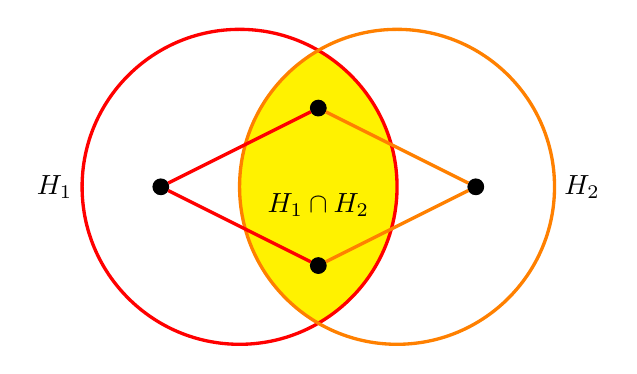
\begin{tikzpicture}[dot/.style = {draw, fill = black, color = black, circle, inner sep=2pt}, >=stealth]
				\begin{scope}
					\clip (-4,0) circle (2);
					\fill [yellow] (-2,0) circle (2);
				\end{scope}
				\draw[very thick, red] (-4,0) circle (2);
				\draw[very thick, orange] (-2,0) circle (2);
				\coordinate[label=left:{$H_1$}] (A) at (-6,0);
				\coordinate[label=right:{$H_2$}] (B) at (0,0);
				\coordinate[label=above:{$H_1\cap H_2$}] (G) at (-3,-0.5);
				\coordinate[dot] (C) at (-5,0);
				\coordinate[dot] (D) at (-1,0);
				\coordinate[dot] (E) at (-3,1);
				\coordinate[dot] (F) at (-3,-1);
				\draw[very thick, red] (C) -- (E) (C) -- (F);
				\draw[very thick, orange] (D) -- (E) (D) -- (F);
			\end{tikzpicture}
		\end{figure}
	
		$H_1$ и $H_2$ связны, $H_1 \cap H_2$ не связен.
		
		\item В стране Семёрка $15$ городов, каждый из которых соединён дорогами не менее, чем с $7$ другими. Докажите, что из любого города можно добраться до любого другого (возможно, проезжая через другие города).
		
		\textbf{Решение}
		
		Докажем от противного.
		
		Предположим, что нельзя, тогда есть минимум $2$ компоненты связности. Так как степень каждой вершины $7$, то они состоят из $8$ городов минимум. $8+8 = 16$, значит все города связаны.
		
		\item Сформулируйте следующее утверждение на языке теории графов и докажите его. На каждой лекции есть два студента, которые знакомы с одинаковом числом студентов (знакомство считается взаимным, если на лекцию пришёл один студент или никто не пришёл -- она отменяется).
		
		\textbf{Решение}
		
		Утверждается, что не существует графа из $N$ вершин в котором степени всех вершин различны. Докажем от противного.
		
		Предположим, что такой граф есть, тогда степени его вершин равны $0,1,2,3,\dots,N-1$. А если есть вершина со степенью $N-1$, то она соединена со всеми вершинами, включая вершину со степенью $0$. Получено противоречие, значит такого графа не существует.
		
		\item Найдите все графы-пути и графы-циклы, дополнение которых граф-путь или граф-цикл.
		
		\textbf{Решение}
		
		Если вершин графа больше $6$ или больше, то степень каждой вершины в полном графе больше либо равна $5$. Тогда дополнение к графу пути или графу циклу будет граф, в котором степень вершины будет минимум $3$, а такого не может быть ни в пути, ни в цикле, значит количество вершин $\textless 6$.
		
		Объединение графа с его дополнением равно полному графу, в котором степени всех вершин равны, значит дополнением пути не может быть цикл и наоборот. 
		
		По этому же принципу у графа с $5$ вершинами под условие подходит только $C_5$, а у графа с $4$ только $L_4$\\
		У $L_3/C_3$ степень всех вершин полного графа 2, значит ни цикл, ни путь не подходит, как и у $L_2$.
		
		\item В новом корпусе МФТИ $15$ аудиторий, каждая из которых соединена прямым переходом не менее, чем с $7$ другими. Докажите, что можно добраться из любой аудитории в любую другую (возможно, транзитом через другие аудитории).

		
		\textbf{Решение}
		
		Предположим, что есть две вершины (аудитории) расположенные в разных компонентах связности. Тогда, чтобы выполнялось условие на количество переходов, в одной компоненте связности должно быть не менее $8$ вершин так как кол-во переходов (ребер, выходящих из одной вершины) должно быть не менее $7$ по условию задачи. Соответственно, так как в одной компоненте связности не менее $8$ вершин, то в двух компонентах связности не менее $16$ вершин. по условию задачи вершин всего $15$. Получаем противоречие.
	\end{enumerate}
	\newpage
	\section{Деревья и раскраски}
	\begin{enumerate}[label={\textbf{\arabic{section}.\arabic*}}]
		\item Степень каждой вершины графа равна $2$. Верно ли, что этот граф $2$-раскрашиваемый?

		
		\textbf{Решение}
		
		Возьмем в качестве примера $C_3$. Все его вершины имеют степень $2$. Однако, если мы попробуем раскрасить его в $2$ цвета, то обязательно на концах одного из ребер будут одинаковые цвета. \textbf{Нет.}
		
		\item Докажите, что в дереве на $2n$ вершинах есть независимое множество размера $n$ (ни одна пара вершин множества не соединена ребром).

		
		\textbf{Решение}
		
		Пользуясь тем, что любое дерево двураскрашиваемое можно предположить, что вершин каждого цвета меньше $n$, тогда во всем графе меньше, чем $2n$ вершин, что противоречит условию. Тогда вершин одного цвета меньше или равно $n$, а второго, наоборот, больше или равно. Из вершин второго цвета можно составить независимое множество.
		
		\item В дереве на $2022$ вершинах ровно три вершины имеют степень $1$. Сколько вершин имеют степень $3$?
		
		\textbf{Решение}
		
		В дереве степень $1$ имеют только конечные вершины листьев. Если
		к конечной вершине добаить еще $2$, то у нее степень станет равна $3$, а количество листьев увеличится на $1$. Не трудно понять, что если сменить степень листа с $1$ на $n$, то кол-во листьев увеличится на $n-2$. В дереве обязательно есть $2$ вершины степени $1$, а в нашем их $3$. Значит, было дабавлено $2$ листа, а один им быть перестал, а это означает, что в нашем дереве ровно $1$ вершина имеет степень $3$.
		
		\item Существуют ли два дерева с одинаковым числом вершин $n$ и одинаковыми диаметрами $d$, такие что можно добавить ребро между вершинами этих деревьев, чтобы длина диаметра полученного дерева равнялась $d$?
		
		\textbf{Решение}
		
		Минимальное расстояние до самой дальней точки дерева из любой
		точки дерева равно $\dfrac{d}{2}$ , т.к. самые дальние друг от друга точки дерева лежат на концах диаметра дерева, если выбранная точка лежит на диаметре, то минимальное расстояние досамой дальней точки дерева – $max(n; dn) \geq \frac{d}{2}$, если не лежит на диаметре, то минимальное расстояние до самой дальней точки дерева – $h + max(n; dn) \geq \frac{d}{2}$, h – расстояние до ближайшей точки на диаметре дерева. Из этого, минимальный диаметр дерева, полученного из соединения двух таких деревьев -- $d + 1$ (в диаметр входит добавленное ребро), т.е. нельзя добавить ребро так, чтобы длина диаметра полученного дерева равнялась $d$.
		
		\item Докажите, что если степень каждой вершины графа не превосходит $d$, то его можно правильно раскрасить в $d + 1$ цвет.
		
		\textbf{Решение}
		
		Рассмотрим нераскрашенную вершину. Выберем для нее тот цвет, который отличается от цвета ее соседей (это можно сделать,так как количество соседей меньше количества цветов). Если у нее нет соседей или они еще не раскрашены, то выбираем любой цвет. В итоге получим правильную раскраску графа.
		
		\item Пусть $G$ -- связный граф, который не является графом-путём и $|V (G)| \textgreater 3$. Докажите, что в $G$ есть три вершины $v_1$, $v_2$, $v_3$, в результате удаления которых вместе со всеми смежными рёбрами, получается
		связный граф $G_0 = G[V \backslash \{v_1, v_2, v_3\}]$.
		
		\textbf{Решение}
		
		Построим основное дерево на исходном графе. У него есть хотя бы один лист, уберем его, получим дерево, в котором снова есть хотя бы один лист, повторим действие дважды, в итоге получим дерево без $3$ листьев, значит оно остается связным, значит граф, на котором оно построено, остается связным.
		
		\item В графе на $100$ вершинах, каждая из которых имеет степень $3$, есть ровно $600$ путей длины $3$. Сколько в этом графе циклов длины $3$?
		
		\textbf{Решение}
		
		Посчитаем минимальное число путей длины $3$ в графе. Зафиксируем какую-то вершину. Из нее ведет $3$ ребра, значит $3$ способа выбрать первое ребро. Далее есть $2$ способа выбрать $2$ ($3$ -- то, по которому пришли). Если путь заканчивается в начальной вершине, то вариант $3$ ребра единственен, значит $6$ вариантов на каждую вершину, значит всего $600$ путей, значит удовлетворяет условию, значит всего циклов $100\cdot3\cdot2 = 600$, но мы посчитали каждый цикл $6$ раз ($2$ раза для каждой из $3$ вершин, так как	обход по циклу можно сделать в две стороны). Значит, циклов длины $3$ будет \textbf{100}.

		
		\item Докажите, что любое дерево $2$-раскрашиваемо (существует правильная раскраска в два цвета).
		
		\textbf{Решение}
		
		Граф $2$ раскрашиваемый если в нем не существует циклов нечетной длины. В дереве в целом не существует циклов, соответственно он $2$-раскрашиваемый.
		
		\item Сколько есть правильных $2$-раскрасок у дерева?
		
		\textbf{Решение}
		
		Подвесим дерево за любую вершину и начнем его раскрашивать. Тогда у нас корень будет одного цвета, следующий слой второго и тп. Тогда у нас будет две раскраски в зависимости от цвета корня.
	\end{enumerate}
	\newpage
	\section{Ориентированные графы}
	\begin{enumerate}[label={\textbf{\arabic{section}.\arabic*}}]
		\item Известно, что в неориентированном графе существует маршрут, проходящий по каждому ребру ровно два раза. Верно ли, что в графе есть замкнутый эйлеров маршрут?
		
		\textbf{Решение}
		
		\textbf{Нет, неверно}, можно привести пример такого цикла.
		
		\begin{figure}[h]
			\centering
			\begin{tikzpicture}[dot/.style = {draw, fill = black, color = black, circle, inner sep=1pt}, >=stealth]
				\coordinate[dot, label=above:{$1$}] (A) at (0,0);
				\coordinate[dot, label=below:{$4$}] (D) at (0,-4);
				\coordinate[dot, label=above:{$2$}] (B) at (-3,3);
				\coordinate[dot, label=left:{$3$}] (C) at (3,3);
				\draw (A) -- (D) (A) -- (B) (A) -- (C);
			\end{tikzpicture}
		\end{figure}
		
		В нём есть маршрут, проходящий по каждому ребру два раза ($1-2-1-3-1-4-1$). При этом замкнутого эйлерового маршрута в нём нет, так как для его существования необходимо, чтобы все вершины имели чётную степень.
		
		\item Выходная (она же исходящая) степень каждой вершины в ориентированном графе на $n \geqslant 3$ вершинах равна $n - 2$. Какое количество компонент сильной связности может быть в этом графе? Укажите все возможные значения.
		
		\textbf{Решение}
		
		Может быть только $1$ или $2$ компоненты сильной связности.
		
		$1$ -- если соединить все вершины последовательно, получится ориентированный цикл порядка $n$, то есть можно направить остальные $n-3$ рёбер из каждой вершины как угодно, компонента связности останется одна.
		
		$2$ -- если выбрать $n-1$ вершин и из каждой направить в каждую, получим степень каждой $n-2$. В оставшуюся вершину не идёт ни одного ребра, поэтому она образует компоненту сильной связости (рёбра из неё можно направить как угодно). То есть всего имеем $2$ компоненты сильной связности -- порядка $n-1$ и $1$.
		
		$3$ и более не может быть, поскольку для этого нужно, чтобы хотя бы $2$ вершины были изолированны от остальных, то есть в них не должно идти ни одно ребро. Однако это невозможно, поскольку изолируя две (или больше) вершин, у нас остаётся $n-2$ (или меньше) вершин, которые все должны быть связаны, но не иметь рёбер, исходящих в эти изолированные вершины (которые, конечно, будут иметь рёбра, исходящие в какие-то из $n-2$ вершин). Такое невозможно, так как у каждой вершины степень $n-2$, значит, она в любом случае будет связана с одной из изолированных вершин и компонент связности будет меньше $3$.
		
		\item В стране некоторые пары городов соединены односторонними прямыми авиарейсами (между любыми двумя городами есть не более одного рейса). Скажем, что город $A$ доступен для города $B$, если из $B$ можно долететь в $A$, возможно, с пересадками. Известно, что для любых двух городов $P$ и $Q$ существует город $R$, для которого и $P$, и $Q$ доступны. Докажите, что существует город, для которого доступны все города страны. (Считается, что город доступен для себя.)
		
		\textbf{Решение}
		
		Рассмотрим город $A$, для которого доступно наибольшее количество городов (если таких несколько -- любой из них). Предположим, что некоторый город $B$ недоступен для $A$. По условию существует город $C$, для которого $A$ и $B$ доступны. Но тогда для $С$ доступны $B$, а также все города, доступные для $A$. Противоречие.
		
		\item В классе учится $15$ мальчиков и $15$ девочек. В день $8$ Марта некоторые мальчики позвонили некоторым девочкам и поздравили их с праздником (никакой мальчик не звонил одной и той же девочке дважды). Оказалось, что детей можно единственным образом разбить на $15$ пар так, чтобы в каждой паре оказались мальчик с девочкой, которой он звонил. Какое наибольшее число звонков могло быть сделано?
		
		\textbf{Решение}
		
		Обозначим мальчиков как $B_1$, $B_2$,$\dots$, $B_{15}$, а девочек -- $G_1$, $G_2$,$\dots$, $G_{15}$. $B1-G1$, $B2-G2$,$\dots$, $B15-G15$ -- разбиение детей по парам. Пусть каждый мальчик позвонил хотя бы двум девочкам. 
		Возмем мальчика $B_i$. Проведем от девочки $G_i$, с которой он в паре, стрелку. Сделаем так для всех мальчиков. Потом от каждого мальчика $B_i$ проведем стрелку к девочке, которой он звонил (не $G_i$). Если мы будем двигаться по стрелкам (начав от произвольной девочки), то рано или поздно мы попадём к девочке, которая уже встречалась в цепочке. Таким образом, в соответствующем графе есть цикл. Объединим в этом цикле каждого мальчика с девочкой, к которой от него ведет стрелка; остальные пары оставим без изменения. Мы получили другое разбиение на пары, что противоречит условию.
		
		Следовательно, найдётся мальчик, который звонил ровно одной девочке. Если отбросить эту пару, число звонков уменьшится не больше чем на $15$ -- максимальное возможное количество звонков этой девочке. После этого снова найдется мальчик, сделавший ровно один звонок одной из оставшихся девочек. Отбросив эту пару, уменьшим количество звонков не более чем на $14$, и т. д. Итого, было сделано не более  $15 + 14 + \dots + 2 + 1 = 120$  звонков.
		
		\item Профессор Рассеянный построил частичный порядок $\textless_P$ для утреннего одевания:
		\begin{itemize}
			\item[] очки $\textless_P$ брюки $\textless_P$ ремень $\textless_P$ пиджак
			\item[] очки $\textless_P$ рубашка $\textless_P$ галстук $\textless_P$ пиджак
			\item[] брюки $\textless_P$ туфли
			\item[] очки $\textless_P$ носки $\textless_P$ туфли
			\item[] очки $\textless_P$ часы
		\end{itemize}
		Постройте линейный порядок на вещах так, чтобы исходный порядок их одевания не был нарушен.
		
		\textbf{Решение}
		
		Изобразим граф. Чёрным цветом рёбра, заданные профессором. Синим -- добавленные исходя из соображений удобства. Тогда есть маршрут Очки-Брюки-Часы-Носки-Туфли-Ремень-Рубашка-Галстук-Пиджак.
		
		\begin{figure}[h]
			\centering
			\begin{tikzpicture}[scale = 0.8, dot/.style = {draw, fill = black, color = black, circle, inner sep=1pt}, >=stealth]
				\coordinate[dot, label=left:{Очки}] (A) at (0,0);
				\coordinate[dot, label=below:{Брюки}] (B) at (5,0);
				\coordinate[dot, label=above right:{Ремень}] (C) at (10,0);
				\coordinate[dot, label=right:{Пиджак}] (D) at (15,0);
				\coordinate[dot, label=below:{Рубашка}] (E) at (2.5,-4);
				\coordinate[dot, label=below:{Галстук}] (F) at (8,-4);
				\coordinate[dot, label=above:{Носки}] (G) at (1.5,4);
				\coordinate[dot, label=above:{Туфли}] (H) at (8.5,4);
				\coordinate[dot, label=right:{Часы}] (I) at (3.25,2);
				\draw[->] (A) -- (E); 
				\draw[->] (A) -- (G); 
				\draw[->] (A) -- (B);
				\draw[->] (A) -- (I); 
				\draw[->] (E) -- (F); 
				\draw[->] (B) -- (C); 
				\draw[->] (F) -- (C); 
				\draw[->] (G) -- (H); 
				\draw[->] (B) -- (H);
				\draw[->] (F) -- (D);
				\draw[->] (C) -- (D);
				\draw[->, blue] (B) -- (I); 
				\draw[->, blue] (I) -- (G);
				\draw[->, blue] (H) -- (C);
				\draw[->, blue] (C) -- (E);
			\end{tikzpicture}
		\end{figure}
		
		\item  Сколько есть порядков на $n$-элементном множестве, в которых ровно одна пара элементов несравнима?
		
		\textbf{Решение}
		
		Отношение порядка можно представить в виде ряда вершин, расположенных слева направо, при этом из любой вершины можно попасть только в вершину правее неё (причём во все вершины правее неё, что следует из транзитивности). Тогда то, что две вершины несравнимы, означает, что они стоят как бы друг под другом. Такая пара должна быть одна.
		
		Получаем количество таких порядков равным [количество способов выбрать два элемента, которые будут входить в пару] * [количество способов расставить оставшиеся элементы] * [количество способов вставить пару между ними], то есть $\dfrac{n \cdot (n-1)}{2} \cdot (n-2)! \cdot (n-1) = \frac{(n-1) \cdot n!}{2}$
		
		\item Докажите, что любой частичный порядок $P$ на конечном множестве $A$ можно продолжить до линейного. То есть можно добавить в $P$ некоторые пары элементов из $A\times A$ так, что любые два элемента $a, b\in A$ окажутся сравнимы: будет выполнено либо $aPb$ либо $bPa$.
		
		\textbf{Решение}
		
		Из условия следует, что если есть $aPb$ и $bPc$, то есть или $aPc$, или $cPa$. В первом случае имеем транзитивное бинарное отношение, то есть отношение порядка строго линейно (так как оно антирефлексивно, антисимметрично и транзитивно). Во втором случае получаем, что есть $aPb$, $bPc$, $cPa$. \textbf{ч.т.д.}
		
		\item Граф $G$ имеет множество вершин $V = \{1, 2, 3, 5, 6, 10, 15, 30\}$. Граф $G$ содержит ребро $\{u, v\}$ (для пределённости $u\textless v$), если $v$ делится на $u$ и не существует (отличной от $v$ и $u$) вершины $s\in V$ , такой что и $v$ делится на $s$ и $s$ делится на $u$.
		\begin{enumerate}[label=\textbf{\alph*)}]
			\item Постройте граф $G$.
			\item Изоморфен ли этот граф булеву кубу $B3$? При положительном ответе укажите биекцию.
		\end{enumerate}
	
		\textbf{Решение}
		
		\begin{figure}[h]
			\begin{minipage}{0.5\linewidth}
				\centering
				\begin{tikzpicture}[scale = 0.76, dot/.style = {draw, fill = black, color = black, circle, inner sep=1pt}, >=stealth]
					\coordinate[dot, label=above left:{$5$}] (A) at (0,0);
					\coordinate[dot, label=above right:{$10$}] (B) at (7,0);
					\coordinate[dot, label=below left:{$1$}] (D) at (0,-7);
					\coordinate[dot, label=below right:{$2$}] (C) at (7,-7);
					\coordinate[dot, label=above:{$10$}] (E) at (2,-2);
					\coordinate[dot, label=above:{$30$}] (F) at (5,-2);
					\coordinate[dot, label=below:{$3$}] (H) at (2,-5);
					\coordinate[dot, label=below:{$6$}] (G) at (5,-5);
					\draw (A) -- (B) (B) -- (C) (C) -- (D) (D) -- (A);
					\draw (E) -- (F) (F) -- (G) (G) -- (H) (H) -- (E);
					\draw (A) -- (E) (B) -- (F) (C) -- (G) (D) -- (H);
				\end{tikzpicture}
			\end{minipage}
			\hfill
			\begin{minipage}{0.49\linewidth}
				\centering
				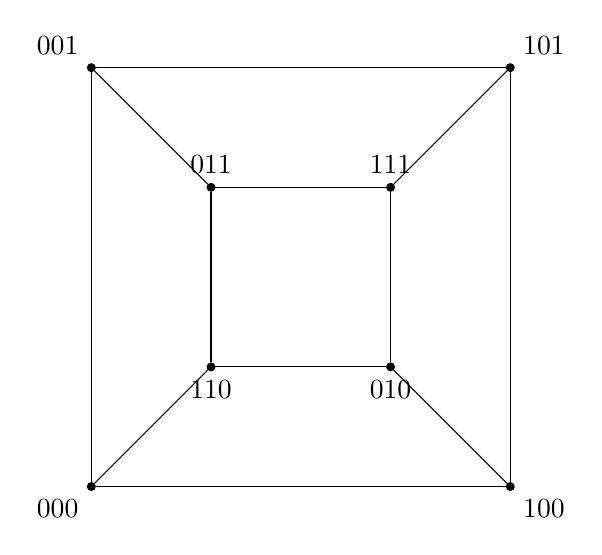
\begin{tikzpicture}[scale = 0.76, dot/.style = {draw, fill = black, color = black, circle, inner sep=1pt}, >=stealth]
					\coordinate[dot, label=above left:{$001$}] (A) at (0,0);
					\coordinate[dot, label=above right:{$101$}] (B) at (7,0);
					\coordinate[dot, label=below left:{$000$}] (D) at (0,-7);
					\coordinate[dot, label=below right:{$100$}] (C) at (7,-7);
					\coordinate[dot, label=above:{$011$}] (E) at (2,-2);
					\coordinate[dot, label=above:{$111$}] (F) at (5,-2);
					\coordinate[dot, label=below:{$110$}] (H) at (2,-5);
					\coordinate[dot, label=below:{$010$}] (G) at (5,-5);
					\draw (A) -- (B) (B) -- (C) (C) -- (D) (D) -- (A);
					\draw (E) -- (F) (F) -- (G) (G) -- (H) (H) -- (E);
					\draw (A) -- (E) (B) -- (F) (C) -- (G) (D) -- (H);
				\end{tikzpicture}
			\end{minipage}
		\end{figure}
		\begin{enumerate}[label=\textbf{\alph*)}]
			\item Граф представлен на рисунке (слева)
			\item Граф \textbf{изоморфен} булеву кубу (это видно в том числе из рисунка). Заметим следущее -- все вершины графа $G$ - это числа, представимые в виде $2^x \cdot 3^y \cdot 5^z$, где $x, y, z$ принимают значение либо $0$, либо $1$. В нашей биекции вершина булева куба - это записанные подряд числа $x, y, z$. Например, $15 = 2^0 \cdot 3^1 \cdot 5^1$, ей соответствует вершина $011$.
		\end{enumerate}
	\end{enumerate}
	\newpage
	\section{Бинарные отношения}
	\begin{enumerate}[label={\textbf{\arabic{section}.\arabic*}}]
		\item Ответьте на следующие вопросы для бинарного отношения $R\subseteq\{1, 2, 3\}\times\{1, 2, 3\}$. Является ли $R$ рефлексивным? симметричным? транзитивным? отношением эквивалентности? Для каждого отношения $R$ нарисуйте соответствующий граф. Используйте неориентированный граф для симметричных бинарных отношений, в случае нерефлексивных бинарных отношений используйте петли.
		\begin{enumerate}[label=\textbf{\alph*)}]
			\item $R = \{(1, 1),(2, 2),(3, 3),(1, 2),(1, 3),(3, 2)\}$
			\item $R = \{(1, 1),(1, 2),(2, 1),(2, 2)\}$
		\end{enumerate}
		
		\textbf{Решение}
		
		\begin{enumerate}[label=\textbf{\alph*)}]
			\item 
			\begin{itemize}
				\item Рефлексивное, так как $1R1, 2R2, 3R3$.
				\item Антисимметричное, так как из 1R2 не следует 2R1.
				\item Транзитивное, так как $\forall a,b,c: aRb, bRc \Rightarrow  aRc$ -- видно из графа.
				\item Не отношение эквивалентности, так как не симметрично.
			\end{itemize}
			\begin{figure}[h!]
				\centering
				\includegraphics[width=0.4\linewidth]{Снимок экрана_20221123_174931.png}
			\end{figure}
			\item 
			\begin{itemize}
				\item Не рефлексивное, так как $3\not R \ 3$.
				\item Симметричное, так как из 1R2 следует 2R1 и наоборот.
				\item Транзитивное, так как $\forall a,b,c: aRb, bRc \Rightarrow  aRc$ -- видно из графа.
				\item Не отношение эквивалентности, так как не рефлексивное.	
			\end{itemize}
			\begin{figure}[h!]
				\centering
				\includegraphics[width=0.4\linewidth]{Снимок экрана_20221123_175026.png}
			\end{figure}
		\end{enumerate}
		
		\item Выразите отношение «племянник(-ца)» через отношения «отец» и «мать» и операции над отношениями.
		
		\textbf{Решение}
		
		Пусть M -- отношение мать, F -- отношение отец.\\
		a,b -- родители b, c; d -- родитель e.\\
		$aMcx, aMd, bFc, bFd \Rightarrow cM^{-1}a, dM^{-1}a, cF^{-1}b, bF^{-1}a$\\
		
		\begin{equation*}
			\begin{cases}
				cM^{-1}a, aMd \Rightarrow c(M\circ M^{-1})d\\
				cF^{-1}b, bFd \Rightarrow c(F\circ F^{-1})d
			\end{cases}
			\Rightarrow (c,d) \in (M\circ M^{-1})\cap (F\circ F^{-1})
		\end{equation*}
		$dMe$ или $dFe$ $\Rightarrow (d,e) \in M\cup F \Rightarrow
		(c,e) \in (M \cap F)\circ (M\circ M^{-1})\cap (F\circ F^{-1})$
		
		\item Пусть бинарные отношения $P_1$, $P_2\subseteq A \times A$ транзитивны. Будут ли $\overline{P_1}$, $P_1\cap P_2$, $P_1\cup P_2$, $P_1\circ P_2$ обладать теми же свойствами?

		
		\textbf{Решение}
		
		$P_1, P_2 \subseteq A\times A$ транзитивные.
		\begin{itemize}
			\item $\overline{P_1}$ -- нет, например для $P_1: (=)$
			\item $P_1 \cap P_2$ -- да, т.к. $a\ P_1\cap P_2 b\ \land c\ P_1\cap P_2\ c = ((aP_1b))\land(bP_2c))\land((aP_2b)\land(bP_2c)) = (aP_1c)\land(aP_2c) = a\ P_1\cap P_2\ c$
			\item $P_1 \cup P_2$ -- нет. Контрпример: $A = {1, 2, 3}; P_1 = {(1,2)}; P_2 = {(2, 3)}$\\
			$R = P_1 \cup P_2 = {(1, 2), (2, 3)}$, но из $1R2$ и $2R3$ не следует $1R3$.
			\item $P_1 \circ P_2$ -- нет. Контрпример: $A = {1, 2, 3, 4, 5}; P_1 = {(2, 3), (4,5)}; P_2 = {(1,2),(3,4)}$\\
			$R = P_1 \circ P_2 = {(1, 3), (3, 5)}$, но из $1R3$ и $3R5$ не следует $1R5$.
		\end{itemize}
	
		\item  Бинарное отношение на множестве из 6 элементов содержит $33$ пары. Может ли оно быть
		\begin{enumerate}[label=\textbf{\alph*)}]
			\item симметричным?
			\item транзитивным?
		\end{enumerate}
	
		\textbf{Решение}
		
		\begin{enumerate}[label=\textbf{\alph*)}]
			\item Может, например отношение, которое содержит все пары кроме $(1,1)(2,2)(3,3)$.
			\item Нет. Пусть отношение транзитивное.\\
			Если среди $36$ возможных пар нет хотя бы одной пары вида $(a,a)$, то так как $\forall b \in {1,2,3,4,5,6}$ из $aPb$ и $bPa$ должно следовать $aPa$ $\Rightarrow \forall$ из $6$ таких пар пар одна из пар должна отсутствовать. Но тогда отсутствует хотя бы $1+6 = 7 \textgreater 3$ пар.
			Если нет хотя бы одной пары вида $(a,b)$, то $\forall b \in {1,2,3,4,5,6}$ из $aPc$ и $cPb$  должно следовать $aPb$ $\Rightarrow \forall$ из $6$ таких пар пар одна из пар должна отсутствовать. Но тогда отсутствует хотя бы $1+6 = 7 \textgreater 3$ пар.\\
			Тогда отношение не транзитивное.
		\end{enumerate}
	
		\item Какие из следующих бинарных отношений на множестве N — отношения эквивалентности?
		\begin{enumerate}[label=\textbf{\alph*)}]
			\item $xPy$ : $у$ чисел $x$ и $y$ одинаковая последняя цифра (здесь и далее в десятичной записи)
			\item $xQy$ : числа $x$ и $y$ отличаются в ровно одной цифре
			\item $xRy$ : разница между суммами цифр $S_x$ и $S_y$ чётна. Формально: пусть $\overline{x_nx_{n-1}\dots x_1x_0}$ -- десятичная запись числа $x$; $S_x = \sum\limits_{k = 0}^n x^k$
		\end{enumerate}
		
		\textbf{Решение}
		
		\begin{enumerate}[label=\textbf{\alph*)}]
			\item Рефлексивное (у $x$ и $x$ последняя цифра одинаковая)\\
			Симметричное (если у $y$ и $x$ одинаковые последние цифры, то и у $x$ и $y$ тоже)\\
			Транзитивное (если у $a$ и $b$ одинаковые последние цифры, у $b$ и $c$ одинаковые последние цифры, то у $a$ и $c$ тоже)\\
			Тогда отношение является отношением эквивалентности.
			\item Не отношение эквивалентности, так как не рефлексивное ($x$ и $x$ отличается в $0$ цифрах).
			\item Рефлексивное, так как $0$ -- четное.\\
			Симметричное, так как если $(a - b)$ четно, то и $(b - a)$ четно, где $a$ и $b$ -- суммы цифр.
			\begin{equation*}
				\begin{cases}
					S_x - S_y \vdots 2\\
					S_y - S_z \vdots 2
				\end{cases}
				\Rightarrow S_x - S_y + S_y - S_z\  \vdots\  2\  \Rightarrow S_x - S_y \ \vdots\ 2
			\end{equation*}
			Т.е. отношение транзитивное.\\
			Тогда отношение является отношением эквивалентности.
		\end{enumerate}
	
		\item Найдите число отношений эквивалентности на множестве $\{1, 2, 3, 4\}$.
		
		\textbf{Решение}
		
		$P$ -- отношение эквивалентности, когда все его классы эквивалентности -- полные графы. Тогда есть $4$ варианта отношения $P$: $1$, $2$, $3$ или $4$ класса.
		
		\begin{figure}[h!]
			\centering
			\includegraphics[width=0.4\linewidth]{Снимок экрана_20221123_195120.png}
		\end{figure}
		\begin{enumerate}
			\item $1$ вариант
			\begin{figure}[h]
				\begin{minipage}{0.5\linewidth}
					\centering
					\includegraphics[width=0.8\linewidth]{Снимок экрана_20221123_195159.png}
				\end{minipage}
				\hfill
				\begin{minipage}{0.49\linewidth}
					\centering
					\includegraphics[width=0.8\linewidth]{Снимок экрана_20221123_195234.png}
				\end{minipage}
			\end{figure}			
			
			\item $4$ способа выбрать изолированную вершину.
		
			\item $6$ способов разбить $4$ элемента на $2$ пары.
			
			\begin{figure}[h!]
				\centering
				\includegraphics[width=0.3\linewidth]{Снимок экрана_20221123_195333.png}
			\end{figure}
		
			\item $1$ способ.
		\end{enumerate}
		Тогда всего получает $1+4+3+6+1 = 15$ вариантов отношений эквивалентности.
		
		\item Об отображениях (всюду определенных функциях) $f$, $g$ из множества $A$ в себя известно, что $f\circ g\circ f = idA$. Верно ли, что $f$ -- биекция? (Множество $A$ не обязательно конечное.)
		
		\textbf{Решение}
		
		$f(g(f(a))) = a \forall a \in A$.
		Предположим $f$ -- не сюръекция $\Rightarrow \exists a \in A : f^{-1}(a) = \varnothing$ 
		$f(g(f(a))) = a; g(f(a)) = b \in A \Rightarrow f(b)  = a \Rightarrow f^{-1}(a) \not = \varnothing$\\ Противоречие.
		Тогда f -- сюръекция. \\
		Пусть f -- не инъекция, тогда $\exists a_1, a_2: f(a_1) = f(a_2)$
		$f(a_1) = f(a_2) \Rightarrow f(g(f(a_1))) = f(g(f(a_2)))$ -- по определению отображения у любого элемента существует ровно один образ $\Rightarrow a_1 = a_2$. Противоречие. Тогда $f$ -- инъекция.\\
		Тогда $f$ -- биекция.
		
		\item Пусть $R$ -- отношение эквивалентности на множестве $A$. Докажите, что существуют такие множество $B$ и отображение $f$ : $A\rightarrow B$, что каждый класс эквивалентности $C$ представим в виде $C = f^{-1}(b)$ для некоторого элемента $b\in B$.
		
		\textbf{Решение}
		
		Построим такое множество $B$ и отображение $f: A \rightarrow B$\\
		Занумеруем все классы эквивалентности и каждому из них сопоставим элемент из $B$, их тоже занумеруем (например, $i$ классу эквивалентности будет соответствовать $i$ элемент из $B$). Тогда $f$ отображение, так как $\forall$  элементу из $A$ соответствует ровно $1$ элемент из $B$ (т.к. классы эквивалентности попарно не пересекаются), а также $ \forall С$ -- класс эквивалентности выполнено: $c_i = f^{-1}(b_i) \Rightarrow$ $B$ и $f$ удовлетворяют условию построения.
		
		\item Множество $A$ состоит из семи элементов. Найдите количество отображений $f$ : $A\rightarrow A$, таких что $f\circ f = idA$.
		
		\textbf{Решение}
		
		Gо доказательству аналогичному $7$ заданию $f$ -- биекция. $f(f(a)) = а$ можно получить в $2$ случаях: $f(a) = a$ или $f(a) = b$, $f(b) = a$, т.е. ввиду биекции у нас элементы либо бьются на пары, либо идут в паре сами с собой. Так как всего элементов $7$ $\rightarrow$ одиночных элементов будет нечетное число (т.к. парных четное), тогда разберем $4$ случая.
		\begin{itemize}
			\item $1$ одиночный элемент. $C_7^1$ -- выбор одного элемента, разбить остальные на три пары -- $5\cdot 3 \cdot 1 = 15$.
			\item $3$ одиночных элемента. $C_7^3$ -- выбор трех элементов, разбить остальные на три пары -- $3$.
			\item $5$ одиночных элементов. $C_7^5$ -- выбор пяти элементов.
			\item $7$ одиночных элементов. $1$ вариант.
		\end{itemize}
		Всего получается $15\cdot 7 + 3\cdot \dfrac{7\cdot 6 \cdot 5}{6} + 21 + 1 = 232$ отображения.
	\end{enumerate}
	\newpage
	\section{Производящие функции}
	\begin{enumerate}[label={\textbf{\arabic{section}.\arabic*}}]
		\item Найдите производящую функцию для последовательности
		\begin{enumerate}[label=\textbf{\alph*)}]
			\item $a_k = k_i$
			\item $a_k = \dfrac{1}{k!}$
		\end{enumerate}
	
		\textbf{Решение}
		
		\begin{enumerate}[label=\textbf{\alph*)}]
			\item Производящая функция имеет вид $1 + 2x + 3x^2 + \dots$. Заметим, что это является производной от функции $C + x + x^2 + x^3 + \dots$. Если взять в качестве $C$ единицу, получим разложение функции $\dfrac{1}{1-x}$ в ряд Тейлора. Значит, искомая производящая функция -- $\dfrac{1}{(1-x)^2}$
			\item Используя формальную запись производящей функции -- $\sum\limits_{k=0}^\infty \frac{x^k}{k!}$ -- видим, что это разложение функции $e^x$. Она и является производящей для этой последовательности.
		\end{enumerate}
	
		\item Выразите аналитически:
		\begin{enumerate}[label=\textbf{\alph*)}]
			\item $\sum\limits_{k\geqslant0}
			\begin{pmatrix}
				n + k \\
				n
			\end{pmatrix} x^k$
			\item $\sum\limits_{k\geqslant0}
			\begin{pmatrix}
				k \\
				n
			\end{pmatrix} x^k$
			\item $\sum\limits_{k=1} (2k+1)x^k$
		\end{enumerate}
	
		\textbf{Решение}
		
		\begin{enumerate}[label=\textbf{\alph*)}]
			\item 
			$$
			\begin{gathered}
				\sum\limits_{k\geqslant0} C_{n+k}^k x^k = \sum\limits_{k\geqslant0} \frac{(n+k)!}{k!n!}x^k = \sum\limits_{k\geqslant0} x^k \frac{(n+1)(n+2)\dots(n+k)}{k!} = \\
				=\sum\limits_{k\geqslant0} (-x)^k \frac{(-n-1)(-n-2)\dots(-n-k)}{k!} = \\
				= \sum\limits_{k\geqslant0} (-x)^k \frac{(-n-1)((-n-1)-1)\dots((-n-1)-(k-1))}{k!} = \\
				=\sum\limits_{k\geqslant0} C_{-n-1}^k (-x)^k = (1-x)^{-n-1} = \frac{1}{(1-x)^{n+1}}
			\end{gathered}
			$$
			\item 
			$$
			\begin{gathered}
				\sum\limits_{k\geqslant0} C_k^n x^k = \sum\limits_{k\geqslant0} \frac{k!}{n!(k-n)!} x^k = \sum\limits_{k\geqslant0} \frac{k(k-1)(k-2)...(k-(n-1))}{n!} x^k
			\end{gathered}
			$$
			
			При $k < n$, в каждом слагаемом найдётся множитель, равный 0, поэтому можно начинать с $k = n$:
			
			$$
			\begin{gathered}
				\sum\limits_{k\geqslant n} C_k^n x^k = \sum\limits_{k\geqslant 0} C_{k+n}^n x^{k+n} = x^n \cdot \sum\limits_{k\geqslant 0} C_{k+n}^n x^{k} = \\
				= \frac{x^n}{(1-x)^{n+1}}
			\end{gathered}
			$$
			\item 
			Возьмём $f(x) = \dfrac{1}{1-x}$
			
			$$
			\begin{gathered}
				f(x) = \sum\limits_{k\geqslant 0} x^k \Rightarrow f'(x) = \sum\limits_{k\geqslant 1} kx^{k-1} \Rightarrow \\
				2xf'(x) = \sum\limits_{k\geqslant 1} 2kx^k
			\end{gathered}
			$$
			
			Тогда
			
			$$
			\begin{gathered}
				\sum\limits_{k\geqslant 1} (2k+1)x^k = 2xf'(x) + xf(x) = \frac{2x}{(1-x)^2} + x\frac{1-x}{(1-x)^2} = \frac{3x - x^2}{(1-x)^2}
			\end{gathered}
			$$
		\end{enumerate}
	
		\item Упростите выражение:
		\begin{enumerate}[label=\textbf{\alph*)}]
			\item $\sum\limits_{k = 0}^n k
			\begin{matrix}
				n \\
				k
			\end{matrix} 2^k)$
		\end{enumerate}
	
		\textbf{Решение}
		
		\begin{enumerate}[label=\textbf{\alph*)}]
			\item Возьмём $x = 2$
			$$
			\sum\limits_{k = 0}^n k C_n^k x^k = x \cdot \sum\limits_{k = 0}^n C_n^k k x^{k-1} = \\
			= x \cdot (\sum\limits_{k = 0}^n C_n^k x^k)^, = x \cdot ((1+x)^n)^, = x \cdot n \cdot (1+x)^{n-1}
			$$
			Подставив обратно 2 вместо $x$, получаем
			$$
			2n3^{n-1}
			$$
		\end{enumerate}
	
		\item Докажите, что $\sum\limits_{k = 2}^n k \cdot (k-1) \cdot \begin{matrix}
			n \\
			k
		\end{matrix} = n \cdot (n - 1) \cdot 2^{n - 2}$
		
		\textbf{Решение}
		
		$$
		k \cdot (k-1) \cdot C_n^k = \frac{k \cdot (k - 1) \cdot n!}{k! \cdot (n - k)!} = n \cdot (n - 1) \cdot \frac{(n - 2)!}{(k - 2)! \cdot (n - 2 - (k - 2))!} = n \cdot (n - 1) \cdot C_{n-2}^{k - 2}
		$$
		
		Тогда
		
		$$
		\sum\limits_{k=2}^n k \cdot (k-1) \cdot C_n^k = \sum\limits_{k=2}^n n \cdot (n - 1) \cdot C_{n-2}^{k - 2} = n \cdot (n - 1) \cdot \sum\limits_{k=2}^n C_{n-2}^{k - 2} = n \cdot (n - 1) \cdot \sum\limits_{m=0}^n C_{n-2}^{m} = n \cdot (n - 1) \cdot 2^{n - 2}
		$$
		
		\item Известна производящая функция $g(x)$ для последовательности $S_n =\sum\limits_{k=0}^n a_k$ частичных сумм последовательности $\{a_k\}$. Выразите через неё производящую функцию для последовательности $\{a_k\}$.
		
		\textbf{Решение}
		
		Так как
		$$
		\begin{gathered}
			S_0 = a_0 \\
			S_1 = a_0 + a_1 \\
			S_2 = a_0 + a_1 + a_2 \\
			... \\
			S_n = a_0 + a_1 + ... + a_n,
		\end{gathered}
		$$
		то
		$$
		a_n = S_n - S_{n-1}
		$$
		$g(x)$ - производящая функция для $S_n \Rightarrow$ коэффициент $S_n$ стоит перед $x_n \Rightarrow S_n = \dfrac{g^{(n)}(0)}{n!}$, т.е. все члены, кроме $S_n$, обнулятся.
		
		$a_n = \dfrac{g^{(n)}(0)}{n!} - \dfrac{g^{(n-1)}(0)}{(n-1)!} \Rightarrow$ производящая функция для $a_k$
		$$
		\sum\limits_{k \geqslant 0} \left(\frac{g^{(n)}(0)}{n!} - \frac{g^{(n-1)}(0)}{(n-1)!}\right) \cdot x^k
		$$
	\end{enumerate}
	\newpage
	
\end{document}